\section{Metrics}
\label{sec:metrics}

With the splits in place (§\ref{sec:benchmark}), we turn to scoring.
Reporting aggregate RMSE works for single-solvent regression but fails
here for four distinct reasons rooted in the multi-solvent structure
of the data.  We characterise those reasons empirically on \scthree{},
then define the five-metric suite we recommend reporting for every
model.

\subsection{Why multi-solvent is different}
\label{sec:multimodal}

\paragraph{Per-solvent location shift.}
Across the \numval{206} cleaned solvents, per-solvent log~S means span
\textbf{\numval{7.98} log units} (minimum \numval{-6.93}, maximum
\numval{+1.05}) --- nine orders of magnitude in equivalent
concentration.  Figure~\ref{fig:solvent_dist} shows the per-solvent
log~S distribution for the top-20 solvents by row count, ordered by
their per-solvent mean.  The densities overlap substantially in the
middle of the range (both water and alcohols contain solutes spanning
most of the dataset's log~S range) but their locations differ by up
to seven log units.

\begin{figure}[t]
\centering
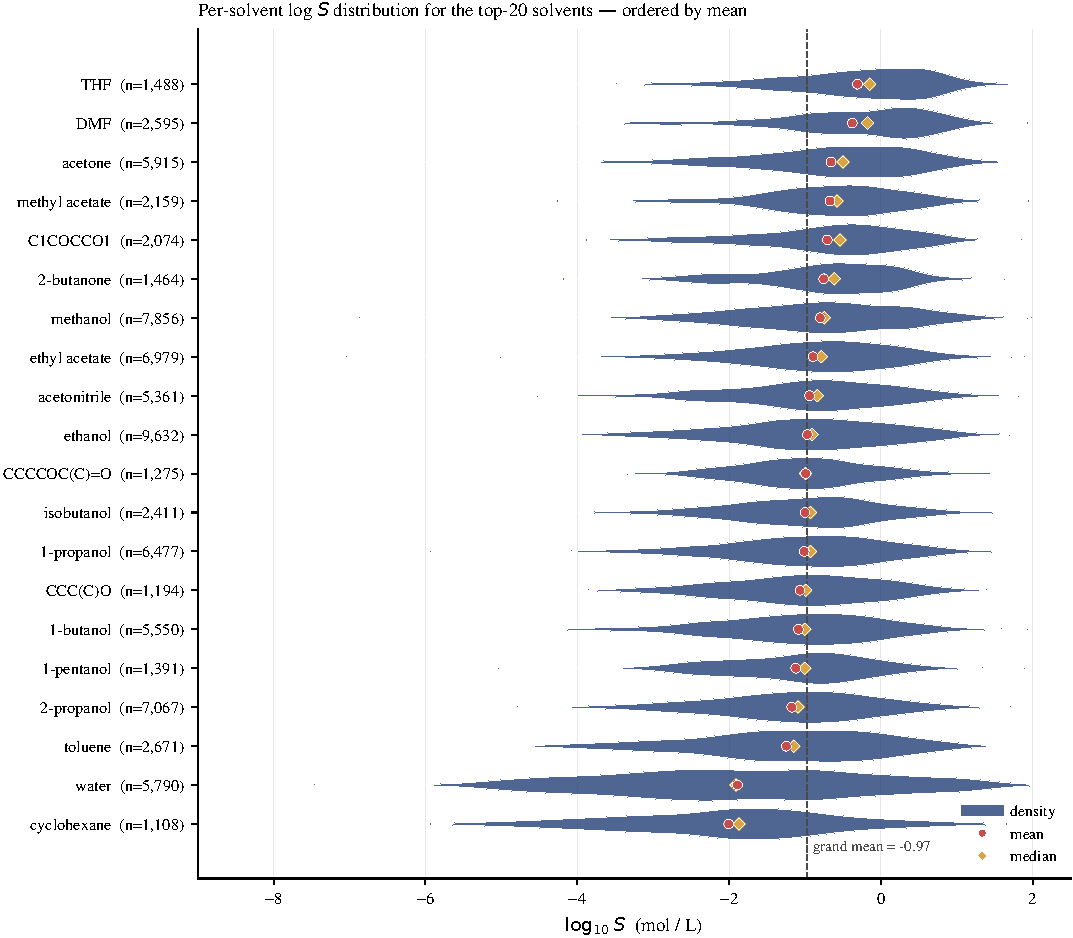
\includegraphics[width=\linewidth]{figures/fig_solvent_distributions.pdf}
\caption{Per-solvent log~$S$ distribution (violin) for the top-20
  solvents by row count, ordered by per-solvent mean.  Red marker =
  mean, gold diamond = median, dashed line = grand mean.  The top-to-
  bottom mean span is $\sim 7$ log~$S$; \emph{any} predictor that
  correctly identifies the solvent absorbs most of that variance for
  free.}
\label{fig:solvent_dist}
\end{figure}

\paragraph{Variance decomposition.}
A one-way ANOVA of cleaned log~S on solvent identity attributes
\textbf{\numval{11.7\,\%}} of total variance to the between-solvent
location shift ($F = \numval{69.9}$ across \numval{206} solvents,
$p < 10^{-300}$).  On OOD, which is built from the long-tail solvents,
the between-solvent fraction rises to \textbf{\numval{22.1\,\%}}
because the long-tail solvents include extremes (e.g.,
1,1-dichloroethane with mean log~S $= -6.93$).  Within each tier the
fraction is closer to \numval{9.3}--\numval{9.9\,\%}.

\paragraph{Dummy-baseline R$^2$.}
We quantify how much of this variance is ``free'' for a trivial model.
A predictor that returns the \emph{per-solvent training mean} (no
solute information, no temperature) achieves the R$^2$ values in
Figure~\ref{fig:dummy_baseline}.  On the in-distribution Eval split,
the baseline scores $R^2 = \numval{+0.053}$ --- positive, non-trivial,
and achievable by a model that only memorises the 25 training-solvent
means.  On the three tiers it scores $R^2 \in [-0.003, +0.017]$, near
zero but within the ID solvent space.  On OOD, where \numval{161} of
\numval{161} test solvents are never seen during training and the
baseline necessarily falls back to the grand training mean, it
\textbf{goes negative} ($R^2 = \numval{-0.062}$) --- the grand mean
is actively worse than no prediction at all on the long-tail solvents.

\begin{figure}[t]
\centering
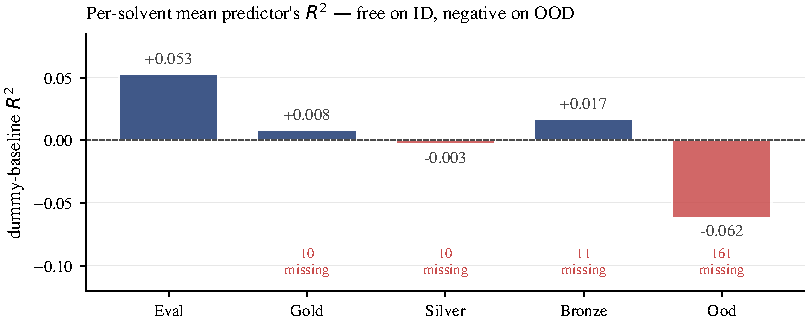
\includegraphics[width=0.75\linewidth]{figures/fig_dummy_baseline.pdf}
\caption{Per-solvent-mean predictor's $R^2$ across the five evaluation
splits.  Positive on in-distribution Eval, near-zero on tiers, and
\emph{negative} on OOD (\numval{161} solvents unseen during training,
so the predictor falls back to the grand mean).  Motivates a metric
suite in which aggregate $R^2$ or RMSE does not reward solvent
identification.}
\label{fig:dummy_baseline}
\end{figure}

\paragraph{Count domination.}
The top-5 solvents (\emph{ethanol, methanol, 2-propanol, ethyl
acetate, 1-propanol}) account for \textbf{\numval{37.5\,\%}} of the
cleaned rows and \textbf{\numval{44.2\,\%}} of Train; the top-25
account for \numval{84.5\,\%} and cover 100\,\% of Train / Eval by
construction.  An aggregate-row metric such as RMSE is therefore,
functionally, a metric on those five solvents.  Reporting only
aggregates would hide per-solvent regression on the long-tail set.

\paragraph{MAPE is broken here.}
\numval{5.6\,\%} of cleaned rows have $|\logS| < 0.1$, and
\numval{28.5\,\%} have $|\logS| < 0.5$ --- the MAPE denominator is
small or zero for a material fraction of the data.  MAPE is therefore
unbounded for any model that makes ordinary-magnitude absolute errors
on these rows and should not be reported as a headline statistic.

\paragraph{Heavy-tailed labels.}
The $|y - \bar{y}|$ distribution has mean/median ratio
$\numval{1.19}$ ($P_{95} = \numval{2.27}$, $P_{99} =
\numval{3.43}$).  RMSE is tail-sensitive in a regime this heavy,
motivating a median absolute error as a robust complement.

\subsection{The SC$^3$ metric suite}
\label{sec:metric_suite}

Combining the above, we define five primary metrics, with
\textbf{PS-RMSE} as the single headline.  Definitions are in
Table~\ref{tab:metrics}.

\begin{table}[h]
\centering\small
\caption{SC$^{3}$ metric suite.  $n$ = rows in the split; $|\mathcal{S}|$
= solvents in the split; $\sigma_i$ = per-row calibrated uncertainty
(tiers only).  The ``applicability'' column lists the splits on which
each metric is computed.  MAPE is reported for diagnostic purposes only.}
\label{tab:metrics}
\begin{tabular}{@{}llcl@{}}
\toprule
Metric         & Formula & Applicability       & Role \\
\midrule
RMSE           & $\sqrt{\frac{1}{n}\sum_i (\hat y_i - y_i)^2}$
               & all
               & count-weighted; baseline \\[1pt]
MAE            & $\frac{1}{n}\sum_i |\hat y_i - y_i|$
               & all
               & less tail-sensitive than RMSE \\[1pt]
MedAE          & $\mathrm{median}_i\,|\hat y_i - y_i|$
               & all
               & robust on heavy-tailed residuals \\[1pt]
\textbf{PS-RMSE} & $\frac{1}{|\mathcal{S}|}\sum_{s\in\mathcal{S}}
                   \mathrm{RMSE}_s$
               & all
               & \textbf{strips count and between-solvent inflation} \\[1pt]
Z-RMSE         & $\sqrt{\frac{1}{n_\sigma}\sum_{i:\sigma_i\ \text{def.}}
                       \bigl((\hat y_i - y_i)/\sigma_i\bigr)^2}$
               & Gold, Silver, Bronze
               & error in units of the aleatoric floor \\[1pt]
\textit{MAPE}  & $\frac{1}{n}\sum_i |\hat y_i - y_i|/|y_i|$
               & \textit{diagnostic}
               & diverges for $|\logS| < \varepsilon$ \\
\bottomrule
\end{tabular}
\end{table}

\paragraph{PS-RMSE.}  Per-solvent RMSE averaged equally across
solvents.  This resolves both the variance-decomposition and
count-domination problems from §\ref{sec:multimodal} in one stroke:
between-solvent location shifts cancel out of the per-solvent RMSE,
and each solvent contributes equally regardless of its row count.
For $|\mathcal{S}|$ large enough, PS-RMSE approaches the
``within-solvent'' RMSE that the ANOVA identifies as the honest
prediction-error variance.

\paragraph{Z-RMSE.}  Error in units of the aleatoric floor.  On rows
where $\sigma_i$ is defined (median \numval{77}\,\% of tier rows,
Table~\ref{tab:tiers}), Z-RMSE $= 1$ means a model is operating at
the measurement-noise limit; Z-RMSE $= 10$ means errors are an order
of magnitude larger than irreducible label uncertainty.  Because
\scthree{} calibrates $\sigma$ per point, Z-RMSE is a
\emph{per-measurement} comparison to the floor, not a comparison to
a single global $\epsA$.

\paragraph{Computational domains.}
Not every metric is computable on every split: Z-RMSE requires
per-row $\sigma$ and is therefore only defined on Gold / Silver /
Bronze, and even there on roughly \numval{77\,\%} of rows.
Table~\ref{tab:metric_domain} reports the effective sample size per
metric per split.

\begin{table}[h]
\centering\small
\caption{Effective sample size per metric per split.  RMSE, MAE, MedAE,
and per-solvent RMSE (PS-RMSE) are computable on every row and every
solvent present in the split.  Z-RMSE is defined only on tier rows
with multi-group consensus ($\sigma$ defined); columns $n_{\sigma}$ and
``Z-coverage'' report the count and fraction accordingly.}
\label{tab:metric_domain}
\begin{tabular}{@{}lrrrrrrr@{}}
\toprule
Split  & rows   & solvents & $n_{\mathrm{RMSE/MAE/MedAE}}$ & $|\mathcal{S}|$ (PS-RMSE) &
         $n_{\sigma}$ & Z-coverage \\
\midrule
Train  & 61\,403 &  25 & 61\,403 &  25 & ---   & ---    \\
Eval   &  6\,969 &  25 &  6\,969 &  25 & ---   & ---    \\
OOD    & 11\,940 & 161 & 11\,940 & 161 & ---   & ---    \\
Gold   &  4\,507 &  26 &  4\,507 &  26 & 3\,449 & 76.5\% \\
Silver &  5\,475 &  27 &  5\,475 &  27 & 4\,212 & 76.9\% \\
Bronze &  6\,331 &  30 &  6\,331 &  30 & 4\,881 & 77.1\% \\
\bottomrule
\end{tabular}
\end{table}

